
\documentclass[sigconf,nonacm]{acmart}
\usepackage{graphicx}

\settopmatter{printacmref=false, printfolios=false}
\setcopyright{none}
\renewcommand\footnotetextcopyrightpermission[1]{}
\pagestyle{plain}
\begin{document}

\title{Preeclampsia Risk Estimation Project Proposal}

\author{Ahmed Khan}
\email{aekhan@ucdavis.edu}
\affiliation{%
  \institution{UC Davis}
  \city{Davis, CA}
  \country{USA}
}

\author{Lawrencedel Legaspi}
\email{lawlegaspi@ucdavis.edu}
\affiliation{%
  \institution{UC Davis}
  \city{Davis, CA}
  \country{USA}
}

\author{Selena Phu}
\email{slphu@ucdavis.edu}
\affiliation{%
  \institution{UC Davis}
  \city{Davis, CA}
  \country{USA}
}

%%
%% This command processes the author and affiliation and title
%% information and builds the first part of the formatted document.
\begin{teaserfigure}
\centering
\resizebox{\textwidth}{!}{%
\begin{tabular}{c}
\url{https://github.com/AhmedKhan-GH/precog_docs}
\ \textbar\ 
\url{https://github.com/AhmedKhan-GH/precog_code}\\[0.2em]
\url{https://docs.google.com/document/d/1VK5gyEvkwuphR05Q0mGYK6_0hERxOEkci-yeKpYLqYA/edit?usp=sharing}
\end{tabular}}
\end{teaserfigure}
\maketitle

\section{Motivation, Background, and Context}
Preeclampsia is a hypertensive disorder in pregnant women that accounts for 2-8\% of pregnancy complications, over 50,000 maternal deaths, and over 500,000 fetal deaths worldwide annually \cite{nbk570611}. According to the World Health Organization, 95\% of deaths occur in low and middle-income countries, and in the United States the financial toll of managing preeclampsia is more than \$2 billion \cite{pmc12364110}. Earlier diagnosis and treatment, especially before the onset of symptoms and complications, can reduce the cost burden and loss of life currently caused by preeclampsia.

  \section{Problem Definition}
Current preeclampsia risk estimation relies on known risk factors, however these do not definitively guarantee development of preeclampsia. Treatment protocols initiate based on complications emerging after 20th week of pregnancy \cite{pmc12364110}. Blanket screening is impractical but the need for definitive evidence delays crucial treatment. Routinely collected data such as ECG waveforms also demand expert analysis, and onset and severity of conditions is often unclear thus still leading to significant morbidity and mortality \cite{pmc12364110}.

\begin{figure}[h]
  \centering
  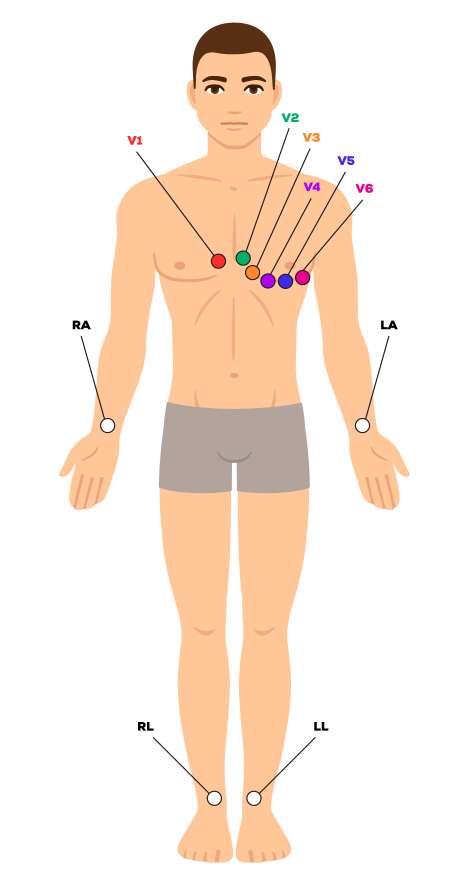
\includegraphics[width=0.48\linewidth]{images/557737215_122141418656891576_230113301145304171_n.jpg}\hfill
  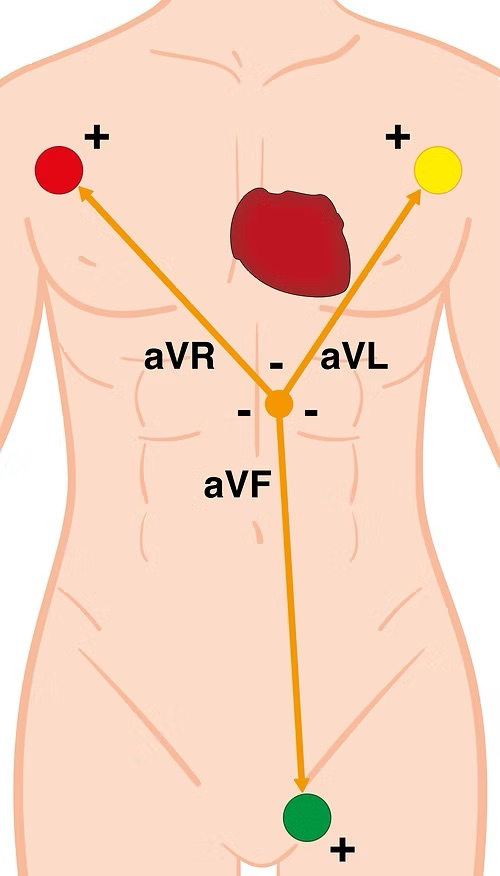
\includegraphics[width=0.48\linewidth]{images/c851b6_fcc62bdd5da74d328afd9dd27e40b2f0-1.jpeg}
  \caption{ECG 12 Leads}
\end{figure}

The problem is a lack of scalable and cost effective risk estimation using available data such as 12-Lead ECG. Machine learning offers such in theory, but accuracy is essential to avoid false negatives. Models demand data and annotated data demands equivalent expert man-hours. Literature reviews indicate the majority of publications around 63\% utilize classic machine learning algorithms which are favoured for their efficiency and ease of implementation, whilst 23\% utilize deep learning, with the remaining percentage as overlap \cite{pmc12364110}. None mention the use of transformers for preeclampsia specifically.

\begin{figure}[h]
  \centering
  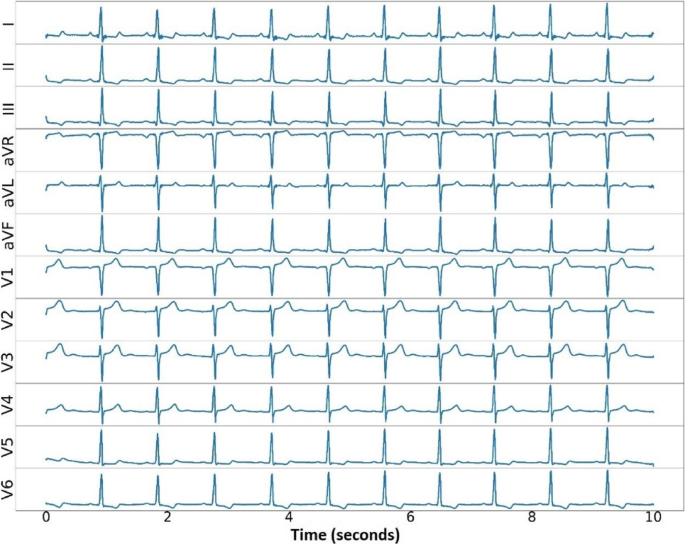
\includegraphics[width=\columnwidth]{images/12911_2023_2233_Fig1_HTML.png}
  \caption{ECG 12 Waveforms}
\end{figure}

  \section{Solution Outline}

\subsection{Transformer Architecture}
The transformer architecture has shown great promise in other areas of medical multivariate timeseries classification, using ECG waveforms to classify cardiovascular diseases with accuracies around 98-99\% \cite{zhao2023transformingecg}. There appears to be a lack of literature for application of transformers for preeclampsia risk estimation from ECG waveform data specifically, thus we aim to do so \cite{zhao2023transformingecg}.
The nature of one-dimensional waveform obscures certain features regarding frequency distribution, we intend to apply time-frequency transforms such as Wavelet or Stockwell that show rich multidimensional representations of one-dimensional data for initial feature extraction by the neural network \cite{kim2025cnntransformer}. Transformers are often paired with 1D or 2D convolutional neural networks for better extraction of local features that can feed into attention maps for long term dependencies.
\cite{zhao2023transformingecg}. Transformers + CNN's may be able to detect and discover features that are otherwise overlooked, leveraging the emergent deep learning properties transformers have shown in other fields.
We will focus on explainability of predictions through visualization tools such as Grad-CAM, and dimensionality reduction through analysis such as PCA to identify which components and features are actually contributing to prediction, and where such is coming from \cite{zhao2023transformingecg}.
\subsection{Feature Extraction}

Feature extraction through signal processing methods is mature and well understood in the field of ECG waveforms, the benefit of which cannot be understated or dispensed with. There is institutional and professional understanding, as well as tools and literature towards the extraction and intrpretation of these features. New workflows must incorporate existing foundations.

Classical machine learning methods such as Random Forest reflect these existing workflows, and they are highly interpretable and explainable. Explainability will be essential for integration into existing clinical workflows to augment expert analysis. A long term responsibility of machine learning in healthcare is to not abandon the human skill in or the reasoning around why a patient has been assigned a certain diagnosis.

Alongside explainability, we will explore model compression of input dimensions and parameter size for deployment on compute constrained edge devices for greater accessibility in compute constrained and data regulated environments.


  \section{Deliverables and Success Criteria}

We will create a deep learning model with CNN + Transformer and other unsupervised methods to increase feature richness We will also create a classical machine learning model with Random Forest trained on featurizations from Neurokit as a baseline. We will benchmark our models on existing public datasets such as Nightingale and MIT-BIH, measuring classification report metrics including UROC, AUCPR, Accuracy, F1-Score, Precision, and Recall.

The model will be accompanied by a purpose-built immediate mode C++ desktop utility named Caliper, built from scratch for real-time deep learning and inference visualization using ImGUI and ImPLOT. It will use Libtorch (Pytorch C++) and graphics visualization OpenGL, both cross-platform GPU accelerated with CUDA on Windows or MPS on MacOS. We will implement efficient data processing with Arrow for efficient retrieval and processing of data. Caliper will be used eventually for visualized diagnosis and feature inference as well as augmented annotation and correction.

We will present a live demonstration of our models dubbed Precog and its associated tool Caliper on the floor of the UC Davis Senior Design Showcase in June 2026, with an interactive demo enabling interested faculty, investors, clinicians, or students to interact with the tools and get a sense for the diagnostic workflow. The project will be accompanied with a slide deck presentation and comprehensive technical report.

  \section{Project Plan}

\subsection{Phase 0}
For onboarding into the research project, we will reproduce the results of Joshi et al.~\cite{joshi2025linkingecgecho}. Their workflow consists of:
\subsubsection{Preprocessing}
Let \(D\in\mathbb{R}^{3751\times 12\times 5000}\) be 3751 ECG waveforms (12 leads each), with labels \(y\in\{0,1\}^{3751}\) for binary preeclampsia classification (\(1=\) preeclampsia, \(0=\) non-preeclampsia).
\[
u:\mathcal{X}\to\mathcal{X}_{\mathrm{bal}},\quad
h:\mathcal{X}_{\mathrm{bal}}\to\mathcal{X}_{\mathrm{hp}},\quad
p:\mathcal{X}_{\mathrm{hp}}\to\mathcal{R},\quad
d:\mathcal{R}\to\mathcal{S},
\]
where \(u\) is random majority undersampling, \(h\) is baseline wander high-pass filtering, \(p=\texttt{ecg\_peaks()}\), \(d=\texttt{ecg\_delineate()}\), and \(\mathcal{S}\) is the featurized heartbeat representation.
\[
\mathcal{S}=(d\circ p\circ h\circ u)(D).
\]

\subsubsection{Featurization}

Let $\mathcal{O}$ be the original feature set with $|\mathcal{O}|=10$:
\{P, PR Segment, PR Interval, PP Interval, RR Interval, QRS Duration, QT Duration, ST Duration, ST-T Duration, TP Interval\}.

Let $\mathcal{E}$ be the extended feature set with $|\mathcal{E}|=6$:
\{ST Elevation, ST Depression, Avg Amp Diff, Med Amp Diff, Max Amp Diff, Min Amp Diff\}.

Let $\mathcal{L}$ be the lead set with $|\mathcal{L}|=12$:
\{I, II, III, aVR, aVF, V1, V2, V3, V4, V5, V6\}.

The total extracted feature index set from $\mathcal{S}$ is $\mathcal{F}=(\mathcal{O}\cup\mathcal{E})\times\mathcal{L}$.
Therefore, $|\mathcal{F}|=(|\mathcal{O}|+|\mathcal{E}|)|\mathcal{L}|=(10+6)\cdot 12=192$.

Define the extraction map $\phi:\mathcal{S}\to\mathbb{R}^{192}$.
Each $s\in\mathcal{S}$ is mapped to a 192-dimensional feature vector indexed by $(f,\ell)\in\mathcal{F}$.

\subsubsection{Random Forest}
Define the Random Forest classifier $f_{\mathrm{RF}}:\mathbb{R}^{192}\to\{0,1\}$, with $y_i=f_{\mathrm{RF}}(\phi(s_i))$ for each $s_i\in\mathcal{S}$.
The model is evaluated using either a default scikit-learn Random Forest or an Optuna-tuned Random Forest (20 trials, TPE sampler).

\subsubsection{1-D Conv. Neural Net}
Define the Convolutional Neural Network classifier $f_{\mathrm{CNN}}:\mathbb{R}^{5000 \times 12}\to\{0,1\}$, with
$y_i=f_{\mathrm{CNN}}(x_i)$ for each ECG input $x_i\in\mathbb{R}^{5000 \times 12}$.
Each block uses $Conv1D(k, s=1, f) \to ReLU \to AvgPool1D(s=2, pool=2)$.

\begin{itemize}
\item Block 1: $k=9, f=64$, output $2500 \times 64$
\item Block 2: $k=9, f=80$, output $1250 \times 80$
\item Block 3: $k=5, f=128$, output $625 \times 128$
\item Block 4: $k=13, f=48$, output $312 \times 48$
\item Block 5: $k=3, f=80$, output $156 \times 80$
\item Block 6: $k=5, f=64$, output $78 \times 64$
\item Block 7: $k=13, f=112$, output $39 \times 112$
\item Block 8: $k=9, f=48$, output $19 \times 48$
\item Block 9: $k=7, f=80$, output $9 \times 80$
\item Block 10: $k=11, f=16$, output $4 \times 16$
\item Block 11: $k=13, f=16$, output $2 \times 16$
\end{itemize}

The classification head is \\
$Flatten \to Dropout(0.7779) \to Dense(35) \to Dense(1)$.

\subsection{Phase 1}
  Working in parallel, we will build two model architectures.

  \subsubsection{Classical Machine Learning}
On our classical machine learning workflow, we will use Neurokit and manual featurization to extract \{Pmax, Pmin, P-wave dispersion, QT Dispersion, Tp-e interval, Tp-e/QT, TP-e/QTc, ST-T abnormalities, Frontal QRS-T angle, QRS Axis, T axis\} and train a classical machine learning model such as Random Forest and performing statistical analysis such as $\chi^2$.

\subsubsection{Modern Deep Learning}
Using Pytorch, we will implement a novel Transformer + Convolutional Neural Network architecture improving on existing research, continuously exploring literature and integrating validated findings. Research and validation will first occur in Python for the sake of automated scripts and hyperparameter tuning. We may use techniques such as undersampling, oversampling, or SMOTE to correct for class imbalance issues if they arise.

  \subsection{Phase 2}
The most successful iteration of the model architecture in Python will be reprogrammed from scratch in C++ and integrated into Caliper, with the aim of modularity such that future models and training architectures can be hot-swapped thereafter. Software engineering best practices and UI/UX principles will be employed to make a production grade clinical workflow improving on existing products.

  \subsection{Phase 3}
We will perform dimensionality reduction through methods such as Principal Component Analysis, to identify the reduced set of ECG leads responsible for providing the relevant diagnostic signals. The rationale being effectiveness under equipment constraint as 12 Lead ECG's though standard are at the upper end of the cost spectrum, and we aim to make an accessible system that can utilize signals captured from substandard settings and situations to assist in regions where the morbidity rate from Preeclampsia is highest due to healthcare resource constraints.

  \subsection{Phase 4}
We will perform model compression techniques through methods such as pruning and quantization to test deployment of the compressed model on compute constrained edge devices. The aim being remote accessibility rather than restricted to powerful compute or cloud compute infrastructure, especially given data privacy regulations and that raw immediate data is restricted from leaving the clinical premises.

  \section{Schedule with Key Milestones}

\begin{table}[H]
\caption{Proposed Project Timeline}
\label{tab:timeline}
\small
\centering
\begin{tabular}{p{0.70\columnwidth}p{0.24\columnwidth}}
\toprule
\textbf{Proposed Activity} & \textbf{Proposed Period} \\
\midrule
Reproduce results from Joshi et al.\ \cite{joshi2025linkingecgecho} & Mar 2--Mar 29 \\
UCDH echo data preprocessing & Mar 30--Apr 5 \\
Feature extraction and feature analysis on data (4/7) & Apr 6--Apr 12 \\
Feature extraction and feature analysis on data (3/7) & Apr 13--Apr 19 \\
KS testing featurization on RF model & Apr 20--Apr 26 \\
Frequency-domain featurization & Apr 27--May 3 \\
Test for reducing required electrodes for preeclampsia detection & May 4--May 10 \\
Test model with Prof.\ Jeong's wearable device & May 11--May 17 \\
Model comparison & May 18--May 24 \\
Slides and report & May 25--May 31 \\
Demo preparation & May 25--May 31 \\
\bottomrule
\end{tabular}
\end{table}

  \section{Resource Allocation and Requirements}
GPU compute is more readily available through our personal gaming machines and thus we do not need to rely on cloud computing, which will perhaps be beneficial given data privacy regulations. We have an RTX 4070, RTX 3090 desktop GPU's and an RTX ADA 500 laptop GPU at our disposal. The desktop GPU's can be dedicated to running large batch jobs in paralellel for fine tuning of hyperparameters and validating different model architectures, whilst the laptop GPU is readily available to do with small-scale experimental configurations on-the-move.

The Nightingale dataset is publicly available and has been provided, however with the UC Davis Health dataset we have yet to encounter or experiment with it, we are uncertain of its size, format, except that it consists  of 1161 data points with 1000 normal cases and 161 preeclampsia cases. Once we are provided it we need to ensure all regulatory guidelines are followed through hard-coded assurances within our continuous integration pipelines such that data can never leave secure channels or permitted devices.

Division of labor will be as follows: Selena and Lawrencedel will work on the Classical Machine Learning model and associated featurizations whilst Ahmed will work on the Deep Learning Model with collaborative use of compute. After the completion of those phases the combination of featurization and inference into visualization will be collaborative. Then finally Lawrencedel and Selena will take charge of Principal Component Analysis on the input data and the feature embedding space, whilst Ahmed will take charge of model compression and validation on edge devices.


\bibliographystyle{ACM-Reference-Format}
\bibliography{sources}
\end{document}
